\section{Rivers \& Streams}

Essential to the realism of virtual rural terrains are water networks. These water networks are constituted of rivers and streams and are the consequence of water being transported by gravity from higher to lower grounds. The algorithm used to model water movement on the terrain is outlined below along with details concerning the GPU implementation.

\subsection{Algorithm Overview}

Precipitation, precipitation intensity and soil infiltration is used to calculate the soil humidity, $S_{h}$ (see equation \ref{eq:monthly_soil_humidity}). The value of which equates to the quantity of water, in millimetres, absorbed by the soil. The standing water, \textit{W$_{standing}$}, is the quantity of water which isn't absorbed by the soil and can be calculated using equation \ref{eq:standing_water_calculation}.\\

\begin{equation} \label{eq:standing_water_calculation}
	W_{standing} = R_{q} - S_{h}
\end{equation}
where:
\begin{itemize}
\item \textit{W$_{standing}$} is the standing water, in millimetres.\\
\item \textit{R$_{q}$} is the monthly rainfall quantity, in millimetres.\\
\item \textit{S$_{h}$} is the quantity of water absorbed by the soil, in millimetres.\\
\end{itemize}

Given the quantity of standing water, W$_{standing}$, for each vertex, a hydrostatic pipe-model similar to that of Stava et al. \cite{StAva2008} is used to determine water movement and build-up on the terrain. The hydrostatic pipe-model works by iteratively attempting to evacuate water from source vertex \textit{V} to any of it's eight surrounding vertices.\\

Although the algorithm is implemented to work in three dimensions where each vertex can evacuate water content to eight surrounding vertices, it also works in a two-dimensional space. With this reduced dimensionality, each vertex \textit{V$_{n}$} has only two surrounding vertices (\textit{V$_{n-1}$} and \textit{V$_{n+1}$}) in which water can be placed. To better grasp the algorithm, it is described for a two-dimensional space. The concept is identical when ported it to a third dimension.  \\

Each vertex \textit{V$_{n}$}, is characterised by it's position (\textit{n}), terrain height (\textit{TerrainHeight$_{n}$}), water height (\textit{WaterHeight$_{n}$}) and absolute height (\textit{AbsoluteHeight$_{n}$} = \textit{TerrainHeight$_{n}$} + \textit{WaterHeight$_{n}$}). Using this data it is possible to calculate the water evacuation capacity, \textit{WEC}, of each terrain vertex (see equation \ref{eq:water_evacuation_capacity}). The value of which effects how much water is evacuated and how it is split amongst surrounding vertices (\ref{subsec:evacuation_approaches}).

\begin{equation} \label{eq:water_evacuation_capacity}
	WEC = 2 \times TerrainHeight_{n} - AbsoluteHeight_{n-1} - AbsoluteHeight_{n+1}
\end{equation}


\subsection{Water Evacuation Approaches} \label{subsec:evacuation_approaches}

Using the water evacuation capacity \textit{WEC} along with table \ref{tab:scenario_based_on_wec}, one of three evacuation approaches are used:  \textit{all water is evacuated}, \textit{a portion of the water is evacuated} or \textit{no water is evacuated}. Each approach is discussed in detail here. \\

\begin{table}[h]
  \centering
	    \begin{tabular}{|p{6cm}|p{3cm}|p{3cm}|p{3cm}|}
		\hline	
  	     &  WEC $>=$ WaterHeight$_{n}$ & 0 $<$ WEC $<$ WaterHeight$_{n}$ & WEC $<$ 0 \\
  	    \hline	
  	    All water can be evacuated & X & - & - \\
		\hline
  	    A portion of water can be evacuated & - & X & - \\
		\hline
  	    No water can be evacuated & - & - & X \\
		\hline
		\end{tabular}
		\caption{Evacuation approach based on water evacuation capacity (\textit{WEC})}
	  \label{tab:scenario_based_on_wec}
\end{table}

\subsubsection{All water is evacuated}

When all water can be evacuated, it is split to surrounding vertices proportionally to their height. This is to model water flowing more intensely on steeper slopes. The quantity of water \textit{W$_{n-1}$} and \textit{W$_{n+1}$} to be evacuated to vertices \textit{V$_{n-1}$} and \textit{V$_{n+1}$} is calculated using equations \ref{eq:all_water_evac_n_minus_one} and \ref{eq:all_water_evac_n_plus_one}. Examples of such situations are illustrated in figure \ref{fig:evacuation_all}. \\

\begin{equation}\label{eq:all_water_evac_n_minus_one}
W_{n-1} = \frac{TerrainHeight_{n} - AbsoluteHeight_{n-1}}{WEC} \times WaterHeight_{n}
\end{equation}

\begin{equation}\label{eq:all_water_evac_n_plus_one}
W_{n+1} = \frac{TerrainHeight_{n} - AbsoluteHeight_{n+1}}{WEC} \times WaterHeight_{n}
\end{equation}

\begin{figure}
\center
	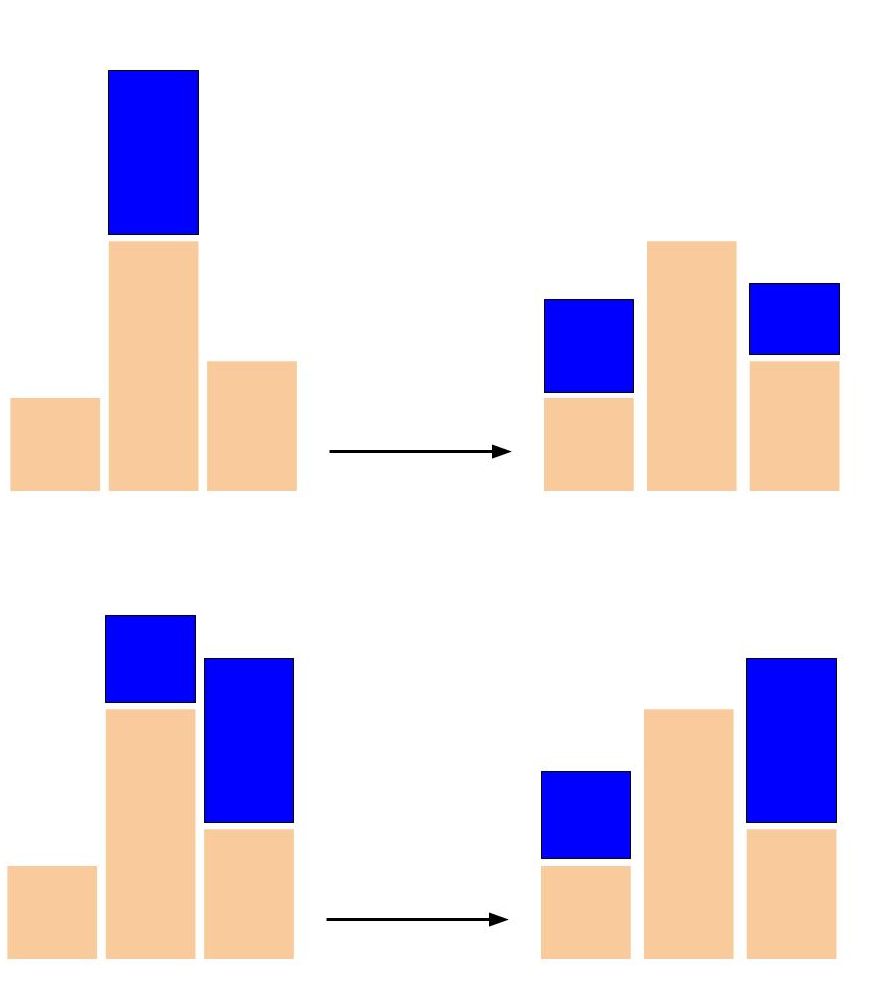
\includegraphics[width=\textwidth/4]{water_evacuation_all.png}
	\caption{ Example water-evacuation scenarios where all water can be evacuated from source vertex (middle).}
	\label{fig:evacuation_all}
\end{figure}

\subsubsection{A portion of water is evacuated}

This approach is used when the water evacuation capacity, \textit{WEC}, is not large enough to purge all water but sufficient to purge a subset thereof. The portion of water which can be evacuated, \textit{W$_{evacuate}$} is calculated using equation \ref{eq:evacuate_calc}. Examples such scenarios are illustrated in figure \ref{fig:evacuation_portion}.

\begin{equation}\label{eq:evacuate_calc}
	W_{evacuate} = AbsoluteHeight_{n} - W_{level}
\end{equation}

Where:
\begin{itemize}
 \item W$_{level}$ is the water level to which water can be evacuated (see equation \ref{eq:water_level_calc}).
\end{itemize}

\begin{equation} \label{eq:water_level_calc}
	W_{level} = \frac{AbsoluteHeight_{n-1} + AbsoluteHeight_{n} + AbsoluteHeight_{n+1}}{3}
\end{equation}

\begin{figure}
\center
	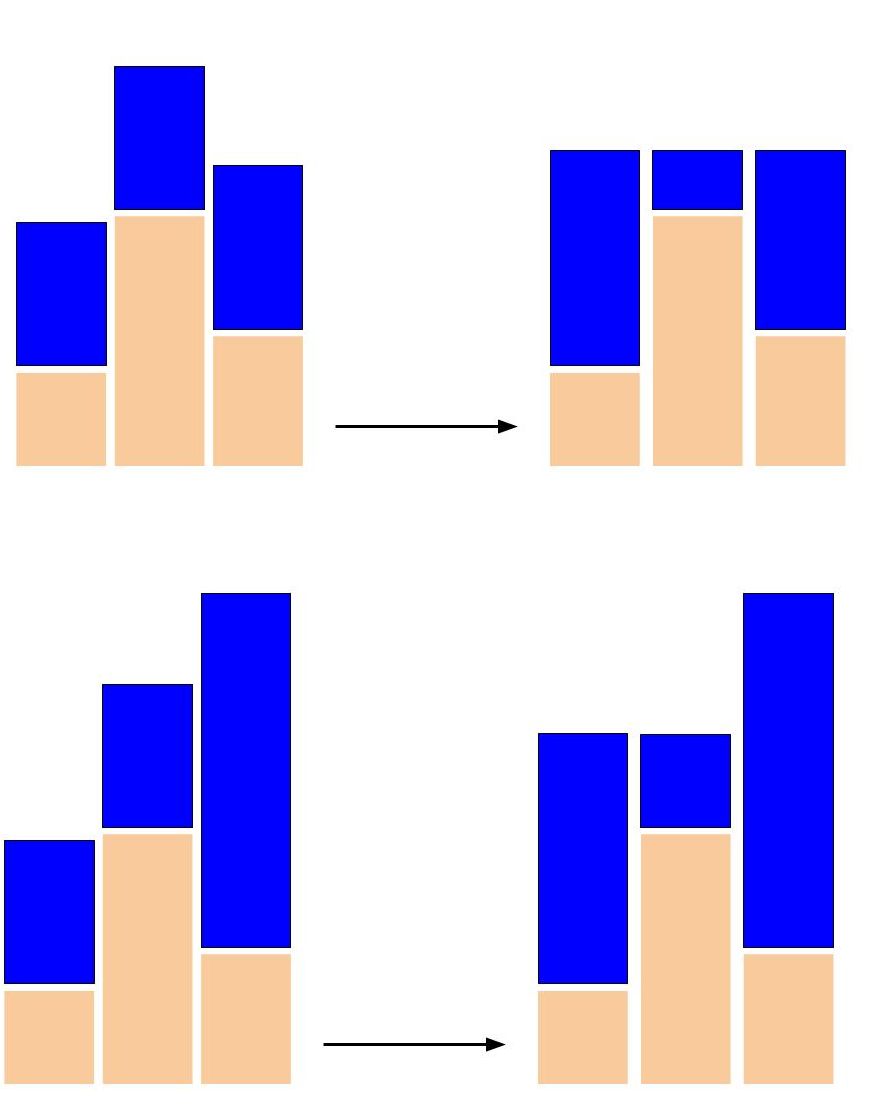
\includegraphics[width=\textwidth/4]{water_evacuation_portion.png}
	\caption{ Example water evacuation scenarios when only a portion of water can be evacuated from the source vertex (middle).}
	\label{fig:evacuation_portion}
\end{figure}

\subsubsection{No water is evacuated}

This situation occurs when there is no capacity for water evacuation and therefore no water can be transported to surrounding vertices. Examples of such scenarios are illustrated in figure \ref{fig:evacuation_all}.

\begin{figure}
\center
	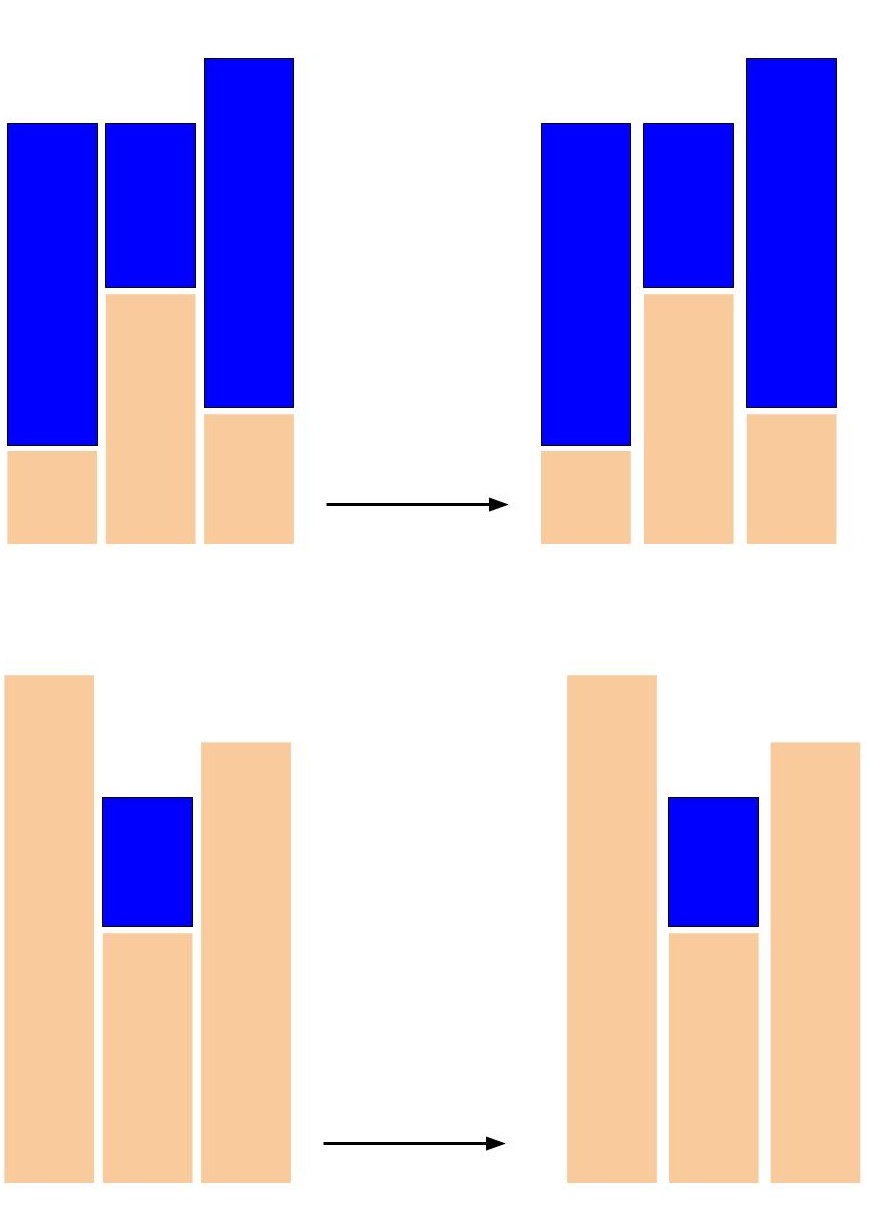
\includegraphics[width=\textwidth/4]{water_evacuation_none.png}
	\caption{ Example water evacuation scenarios where no water can be evacuated from the source vertex (middle).}
	\label{fig:evacuation_none}
\end{figure}

\subsection{Terrain Extremities}

When attempting to evacuate water from vertices on the terrain extremities, one or multiple vertices are missing. One way to deal with this would be to discard those vertices and permit water to flow only to existing surrounding vertices. By employing this approach, however, water would never leave the terrain and could build-up unrealistically. To overcome this, a one vertex thick border is generated around the terrain as illustrated in figure \ref{fig:evacuation_border}. The height of each border vertex is calculated such that the slope remains unchanged. During the water-flow simulation, water is permitted to evacuate to border vertices but water cannot build-up on them.

\begin{figure}
\center
	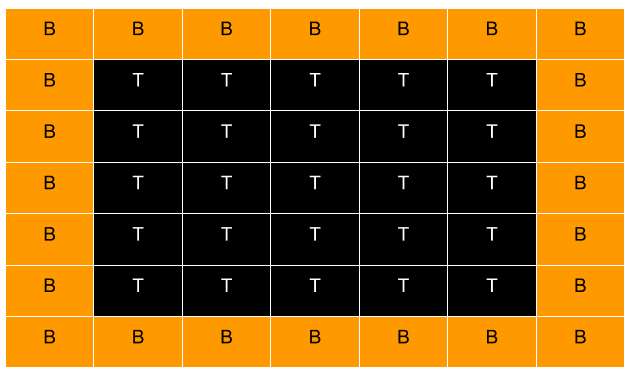
\includegraphics[width=\textwidth]{water_evacuation_border.png}
	\caption{ Border of vertices generated around the terrain to cater for water evacuation at the extremities. Orange vertices form the border. }
	\label{fig:evacuation_border}
\end{figure}

\subsection{Stopping the simulation}

The flow of water on the terrain can be measured by keeping track of the number of vertices which were completely purged at a given iteration of the simulation. This flow will tend to be much larger at the start of the simulation when water is being evacuated from higher grounds and will gradually decrease as water starts to build up and less vertices are able to purge their water content entirely. By also keeping track of the aggregated water flow of all previous iterations of the simulation, it is possible to analyse the evolution of water-flow. The system automatically stops the simulation when the water-flow calculated at iteration \textit{n} is less than one thousandth of the total aggregated water flow during the course of the simulation. \\

The user is able to override this, however, if he wishes to model a different water network which requires a shorter or longer water-flow simulation. 

\subsection{GPU Implementation}

Processing the water flow on the terrain is computationally expensive as the amount of water to evacuate needs to be calculated iteratively for all terrain vertices. To accelerate this process and  process a parallel implement

When processing a single vertex, water can not be removed from surrounding vertices

Both the standing water and the water evacuation algorithm was implemented on the GPU

through the evacuation of run-off water from higher to lower altitudes and, eventually, 

Water networks form due to the evacuation of 
